\subsubsection{Naive Bayes}

A classificação Naive Bayes é um algoritmo de aprendizado de máquina supervisionado que utiliza o teorema de Bayes para classificar instâncias em classes discretas. A principal vantagem do algoritmo Naive Bayes é a sua simplicidade e eficiência computacional, o que o torna uma escolha popular para problemas de classificação em grande escala \citep{mitchell1997machine}.

O algoritmo Naive Bayes é baseado no teorema de Bayes, que fornece uma maneira de calcular a probabilidade condicional de uma hipótese, dado um conjunto de evidências. Na classificação, a hipótese corresponde à classe da instância e as evidências correspondem às características observadas da instância. O algoritmo calcula a probabilidade condicional de cada classe, dado as características observadas da instância, e atribui a instância à classe com a maior probabilidade condicional.

Segundo \cite{domingos1997optimality}, a principal suposição por trás do algoritmo Naive Bayes é a independência condicional das características, ou seja, cada característica contribui independentemente para a probabilidade condicional de cada classe. Embora essa suposição seja muitas vezes violada na prática, o algoritmo Naive Bayes ainda funciona bem em muitos casos e pode ser especialmente útil quando há muitas características.

O algoritmo Naive Bayes tem sido aplicado em muitas áreas, incluindo reconhecimento de fala, processamento de texto e detecção de spam de e-mail. É particularmente útil em aplicações onde há muitas características e as instâncias são discretas ou categóricas. Um estudo empírico sobre o desempenho do algoritmo Naive Bayes em diferentes conjuntos de dados pode ser encontrado em \citep{rish2001empirical}.

Embora o algoritmo Naive Bayes seja uma técnica de classificação simples e eficiente, ele também tem algumas limitações. Por exemplo, a suposição de independência condicional das características pode ser inadequada em algumas situações, e a performance do algoritmo pode ser afetada por dados ausentes ou dados ruidosos \citep{mitchell1997machine}.

As equações abaixo representam a base matemática do algoritmo de classificação Naive Bayes:

Dada uma instância $X = {x_1, x_2, \dots, x_n}$ com características observadas, o objetivo do algoritmo é determinar a probabilidade condicional $P(C_k|X)$ da instância pertencer a cada classe $C_k$.

O teorema de Bayes fornece uma maneira de calcular a probabilidade condicional $P(C_k|X)$ em termos das probabilidades a priori $P(C_k)$ e das probabilidades condicionais $P(X|C_k)$, como segue:

\begin{equation}
    P(C_k|X)=\frac{P(X|C_k)P(C_k)}{P(X)}
\end{equation}

Aqui, $P(C_k)$ é a probabilidade a priori da classe $C_k$ e $P(X|C_k)$ é a probabilidade condicional de observar a instância $X$ dada a classe $C_k$.

O classificador Naive Bayes assume a independência condicional das características dadas a classe, isto é, $P(x_i|C_k, x_1, \dots, x_{i-1}, x_{i+1}, \dots, x_n) = P(x_i|C_k)$. Isso permite simplificar a probabilidade condicional $P(X|C_k)$ como:

\begin{equation}
    P(X|C_k)=P(x_1, \dots, x_{i-1}, x_{i+1}, \dots, x_n|C_k)=\prod_{i=1}^{n}P(x_i|C_k)
\end{equation}

Substituindo essa expressão na equação anterior, tem-se:

\begin{equation}
    P(C_k|X)=\frac{\prod_{i=1}^{n}P(x_i|C_k)P(C_k)}{P(X)}
\end{equation}

Como a probabilidade $P(X)$ é constante para todas as classes, é possível comparar apenas as probabilidades $P(C_k)\prod_{i=1}^n P(x_i|C_k)$ para determinar a classe mais provável para a instância $X$.

O desenho ilustra as variáveis aleatórias $x_1, x_2, x_3, x_4$ e a classe $C_k$. As setas que partem das probabilidades condicionais e a priori indicam as fórmulas para o cálculo das probabilidades conjuntas $P(x_1, x_2, x_3, x_4, C_k)$ e, consequentemente, para a classificação de uma instância.

\begin{figure}[H]
    \centering
    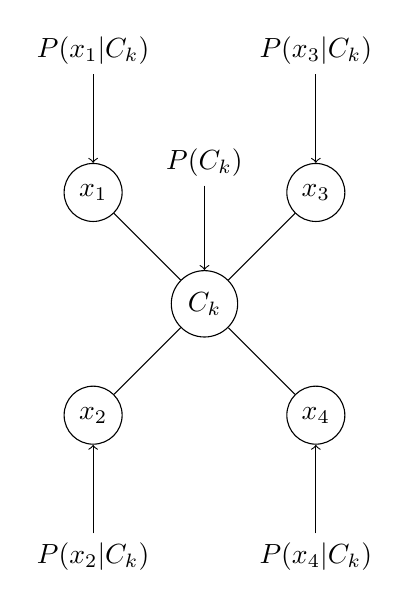
\begin{tikzpicture}[node distance=2cm, auto]
        % Define os nós
        \node[draw, circle] (C) {$C_k$};
        \node[draw, circle, above left of=C] (X1) {$x_1$};
        \node[draw, circle, below left of=C] (X2) {$x_2$};
        \node[draw, circle, above right of=C] (X3) {$x_3$};
        \node[draw, circle, below right of=C] (X4) {$x_4$};
        % Conecta os nós
        \draw[-] (X1) -- (C);
        \draw[-] (X2) -- (C);
        \draw[-] (X3) -- (C);
        \draw[-] (X4) -- (C);
        % Adiciona as probabilidades condicionais
        \node[above of=X1, yshift=-0.2cm] (px1ck) {$P(x_1|C_k)$};
        \node[below of=X2, yshift=0.2cm] (px2ck) {$P(x_2|C_k)$};
        \node[above of=X3, yshift=-0.2cm] (px3ck) {$P(x_3|C_k)$};
        \node[below of=X4, yshift=0.2cm] (px4ck) {$P(x_4|C_k)$};
        % Adiciona as probabilidades a priori
        \node[above of=C, yshift=-0.2cm] (pck) {$P(C_k)$};
        % Adiciona as setas com as fórmulas
        \draw[->] (pck) -- (C);
        \draw[->] (px1ck) -- (X1);
        \draw[->] (px2ck) -- (X2);
        \draw[->] (px3ck) -- (X3);
        \draw[->] (px4ck) -- (X4);
    \end{tikzpicture}
    \caption{Esquema de funcionamento da classificação Naive Bayes}
    \label{plt:bayes}
\end{figure}